

The following series of images are the solutions generated by the Elastic Neighbourhood for each of the tours in the Art TSP dataset \cite{ArtTSP}. These pieces are a wonderful intersection between art and science and demonstrate that creativity can flourish in the bounds analytical methodology. They are generated by the excellent method of Bosch and Kaplan (2005) \cite{bridges2005301}. I highly encourage looking at each of their work: at \href{https://www2.oberlin.edu/math/faculty/bosch/tspart-page.html}{https://www2.oberlin.edu/math/faculty/bosch/tspart-page.html} and \href{https://isohedral.ca/}{https://isohedral.ca/}. My personal favourite in the following collection is \textit{The Desperate Man} by Courbet.
\newpage
\section*{da Vinci's Mona Lisa}
\begin{figure}[h!]
	\centering
	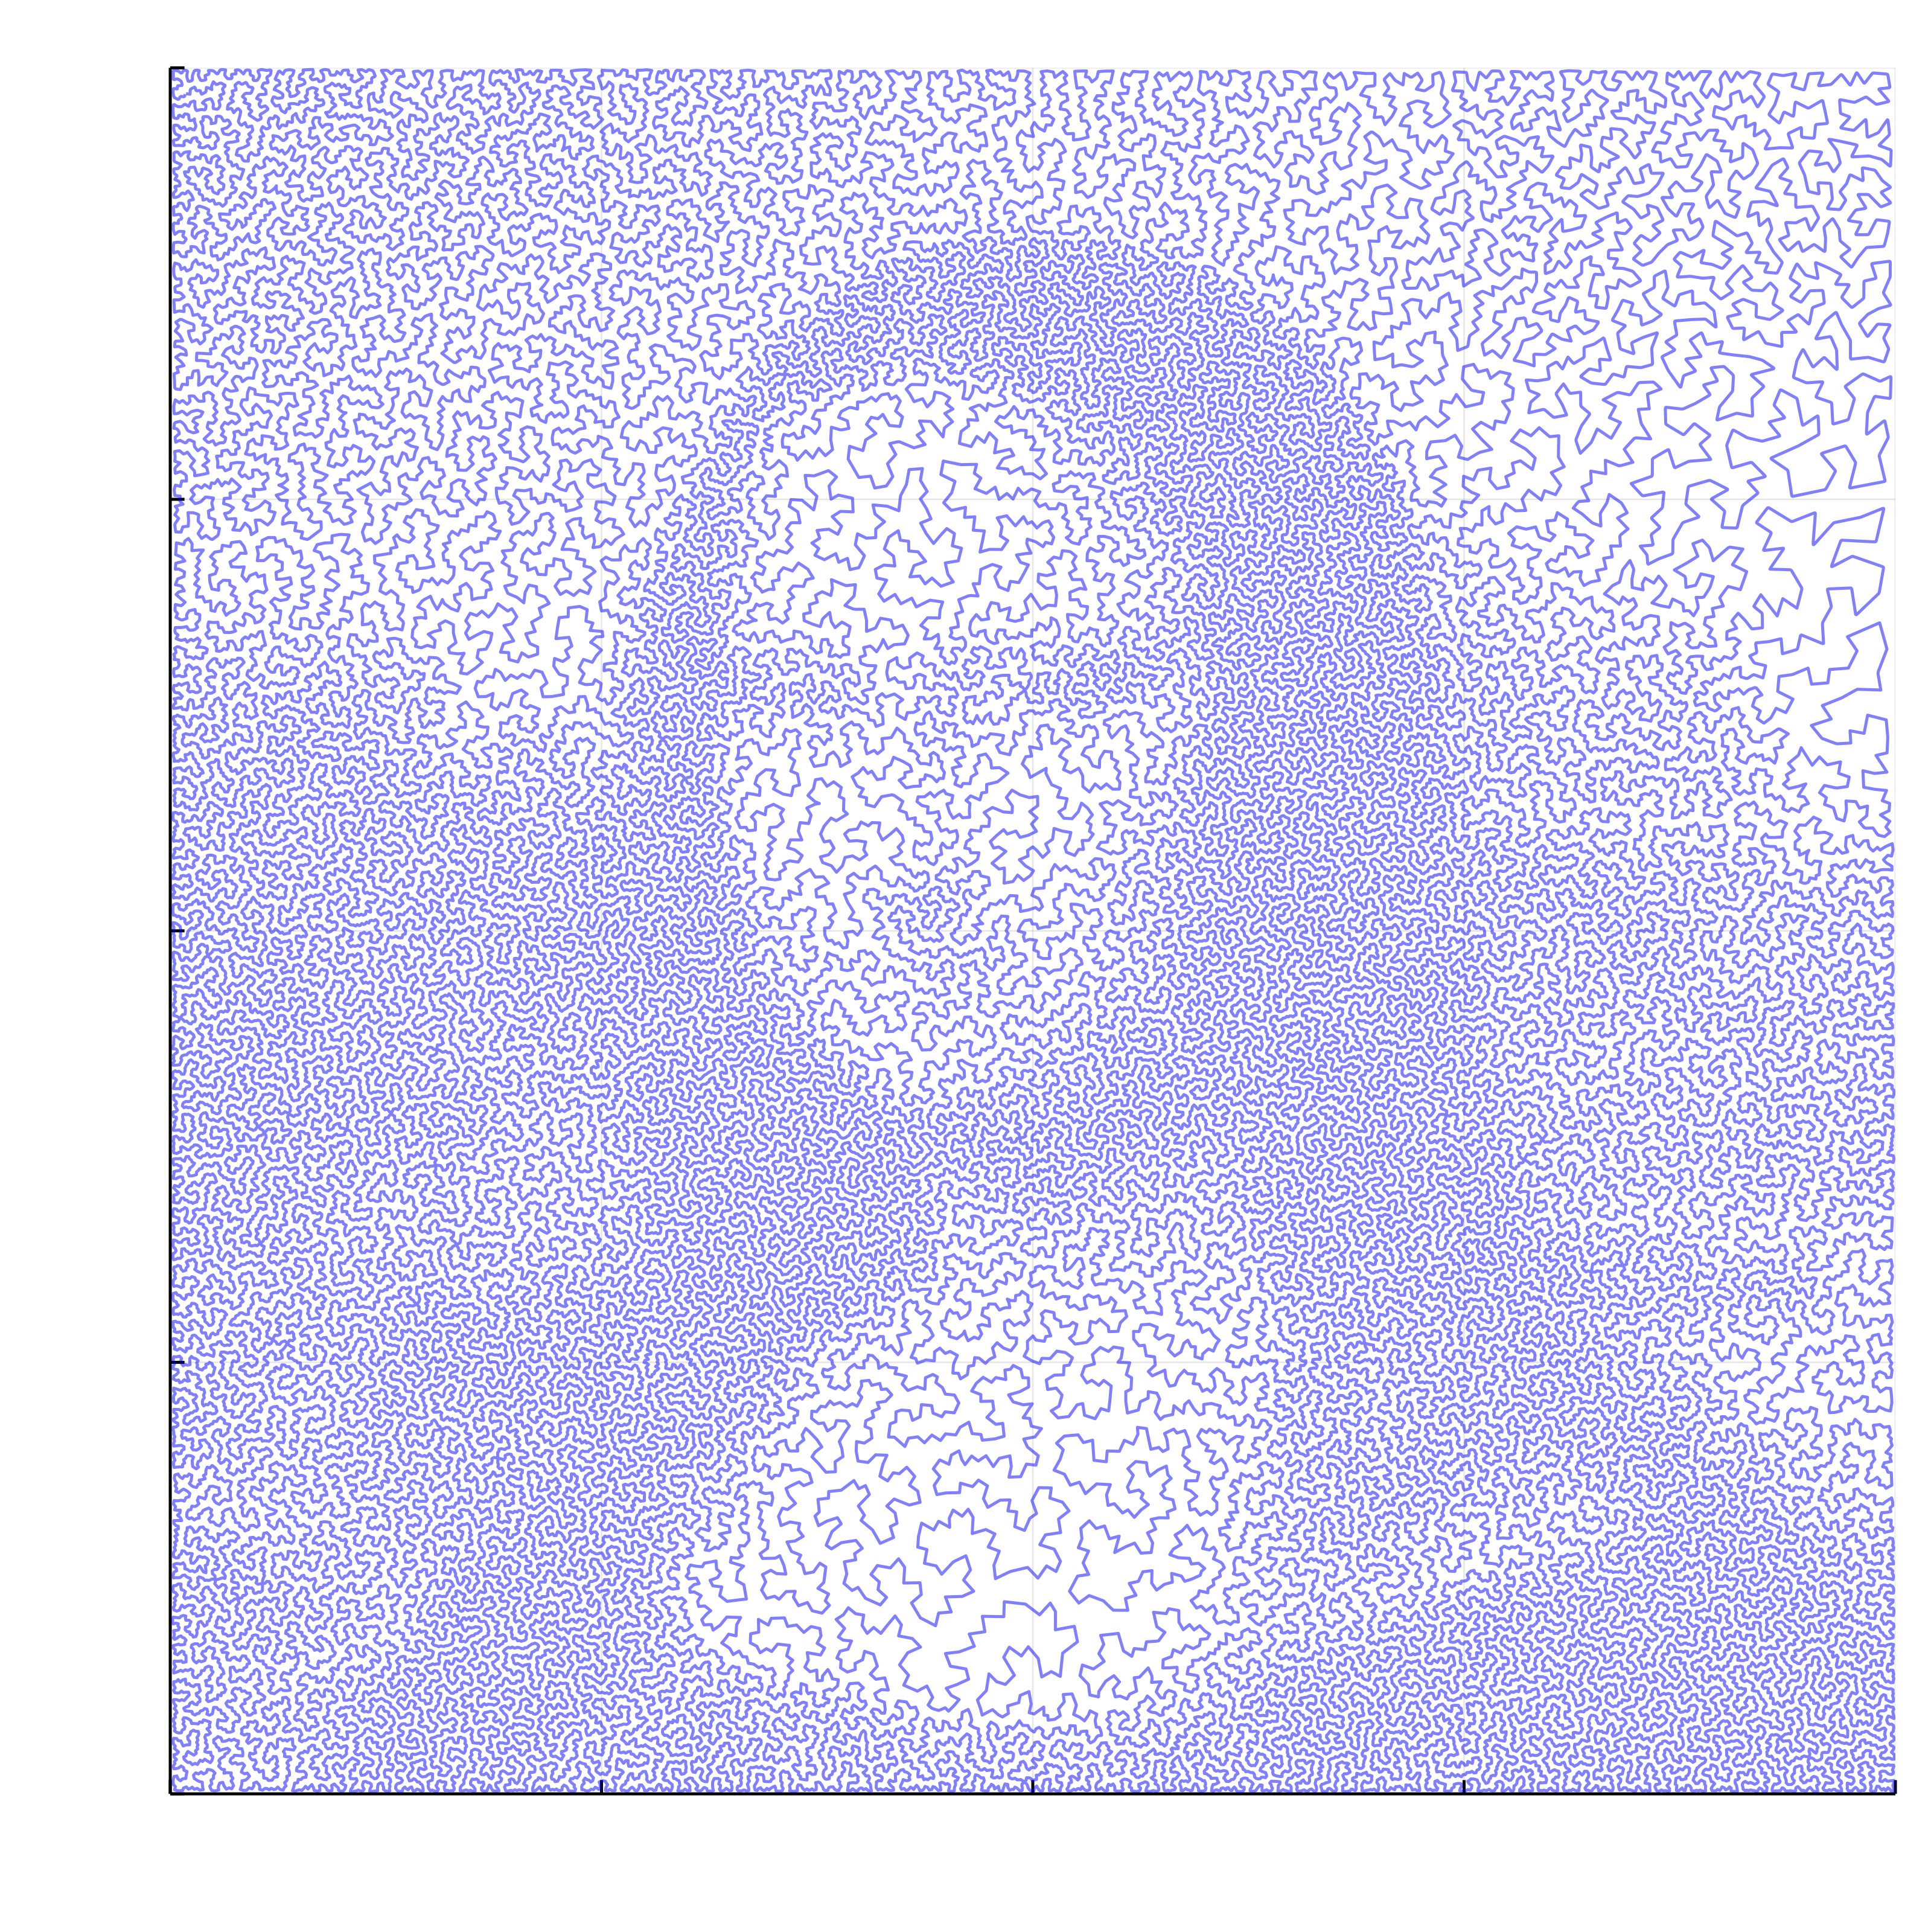
\includegraphics[width=\textwidth]{images/elastic_neighbourhood/fig_1}
\end{figure}
\newpage
\section*{van Gogh's Self Portrait 1889}
\begin{figure}[h!]
	\centering
	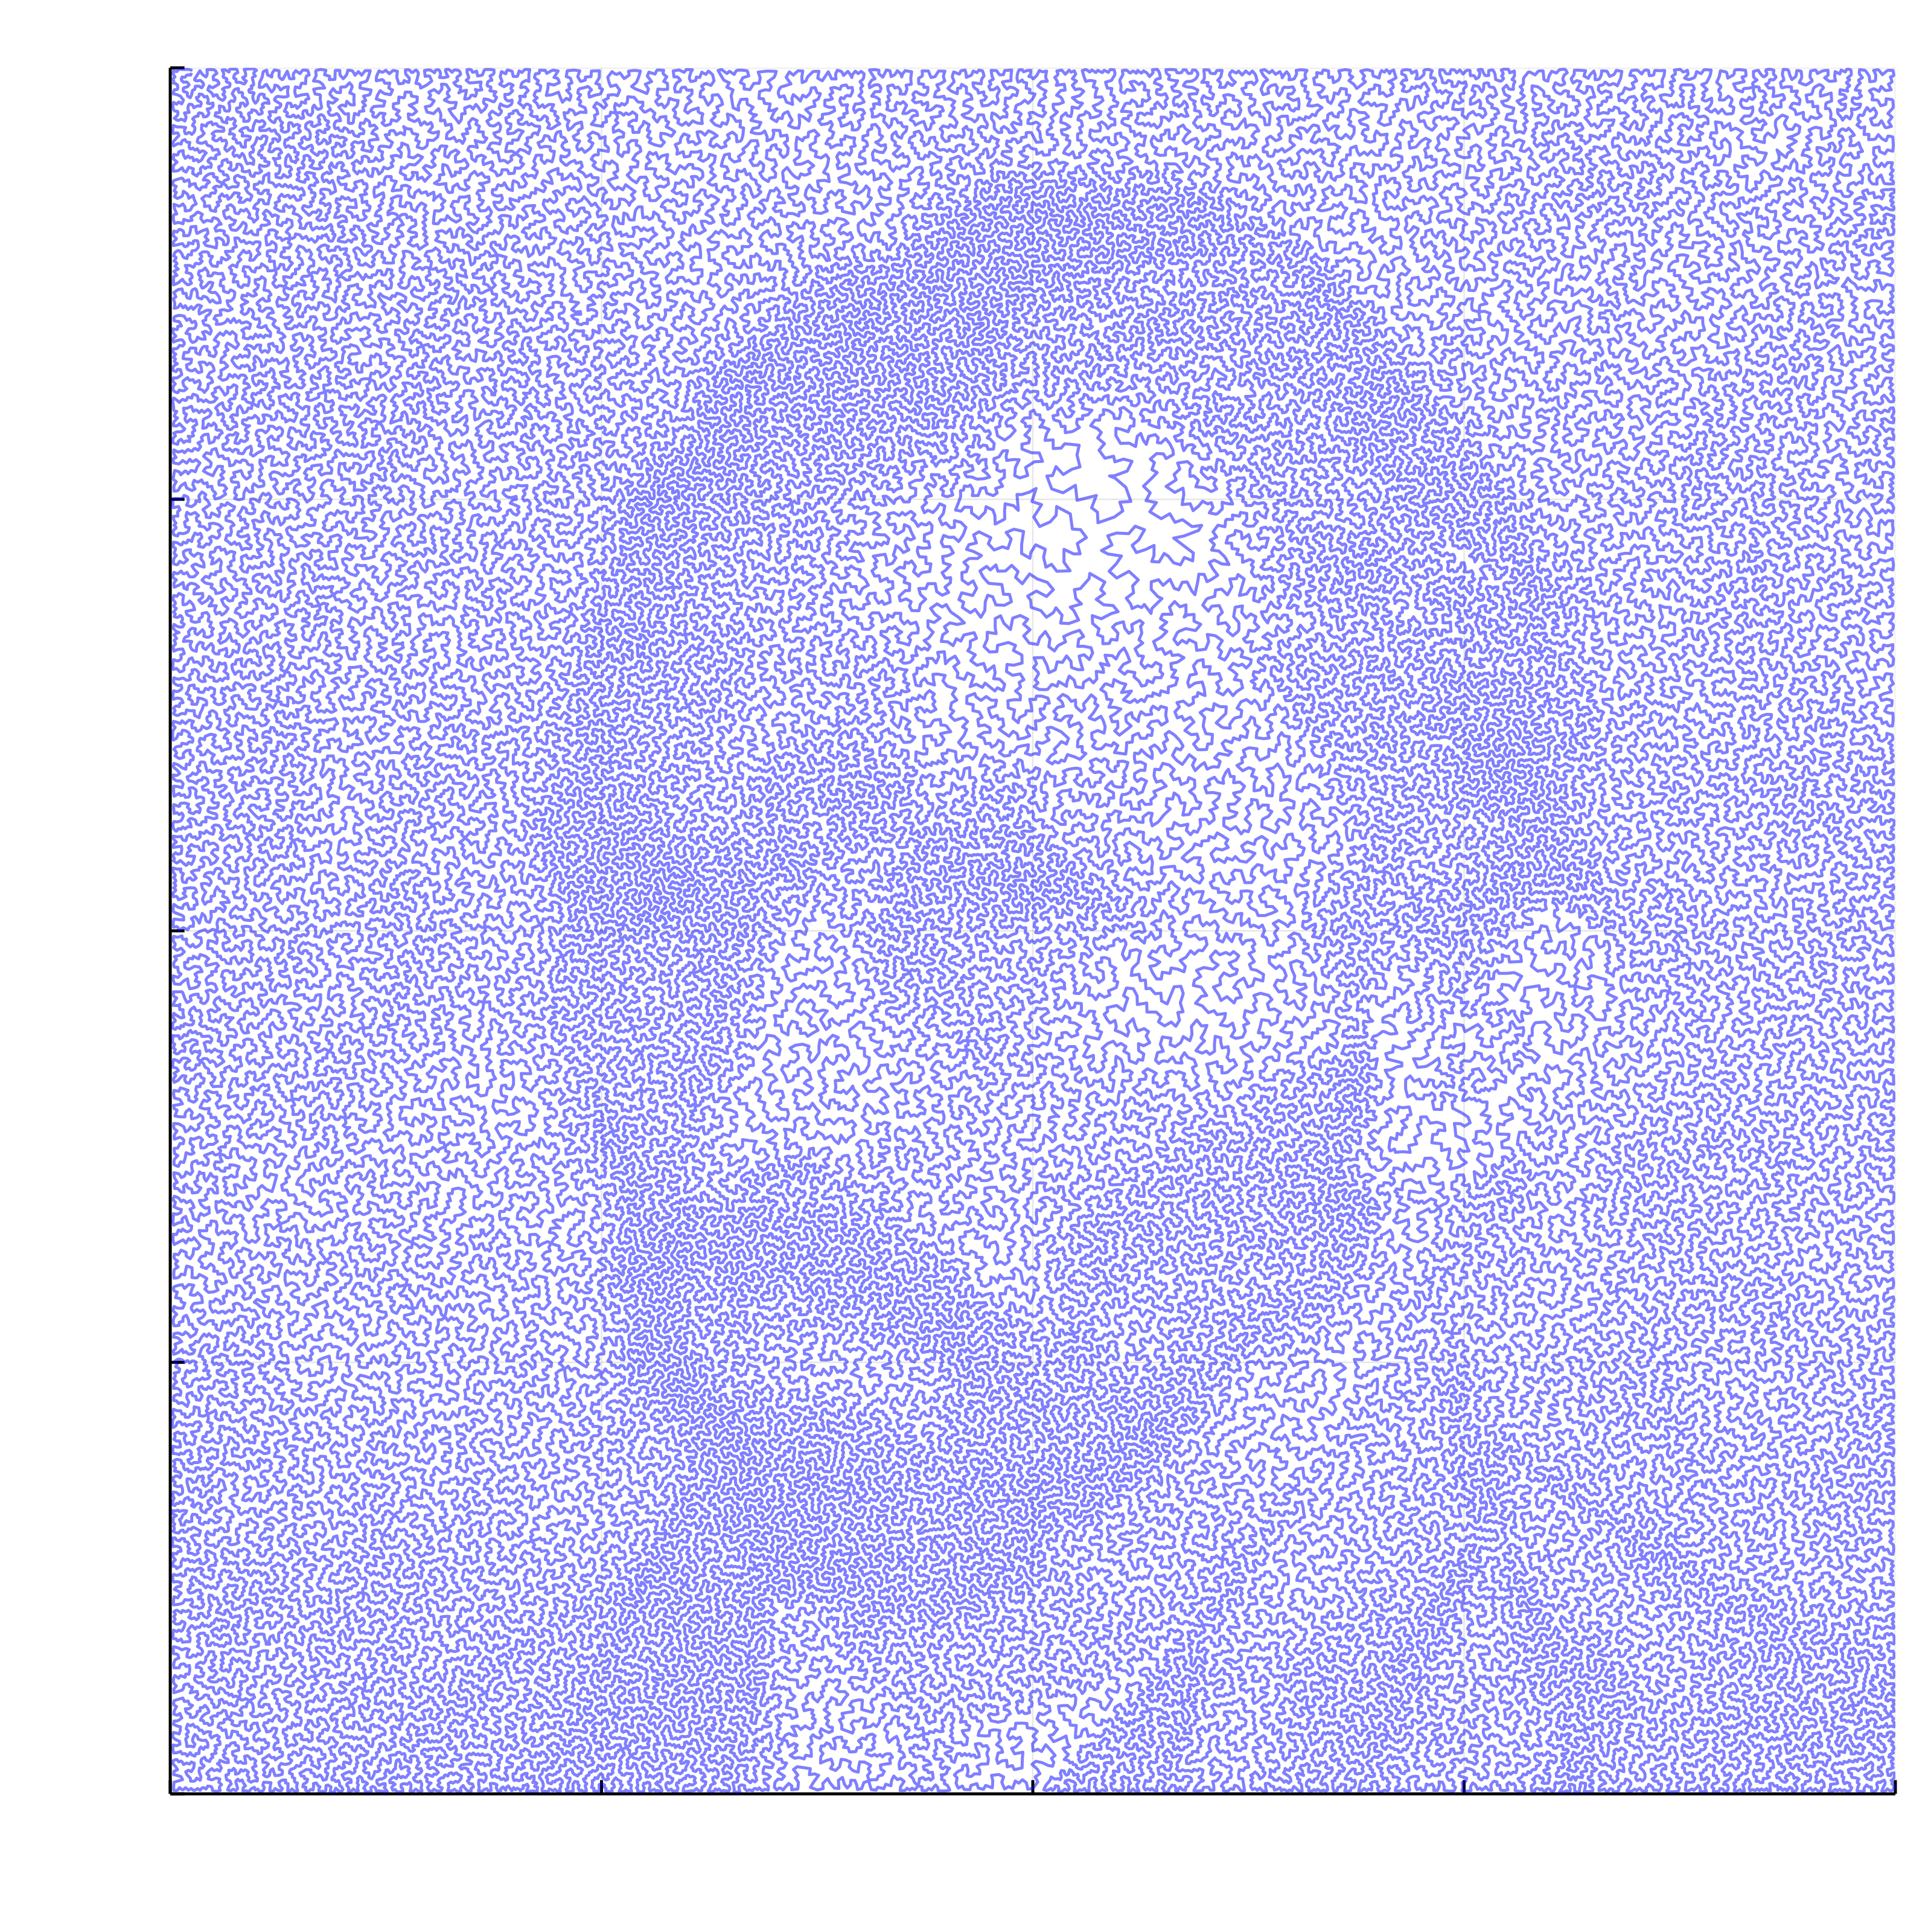
\includegraphics[width=\textwidth]{images/elastic_neighbourhood/fig_2}
\end{figure}
\newpage
\section*{Botticelli's The Birth of Venus}
\begin{figure}[h!]
	\centering
	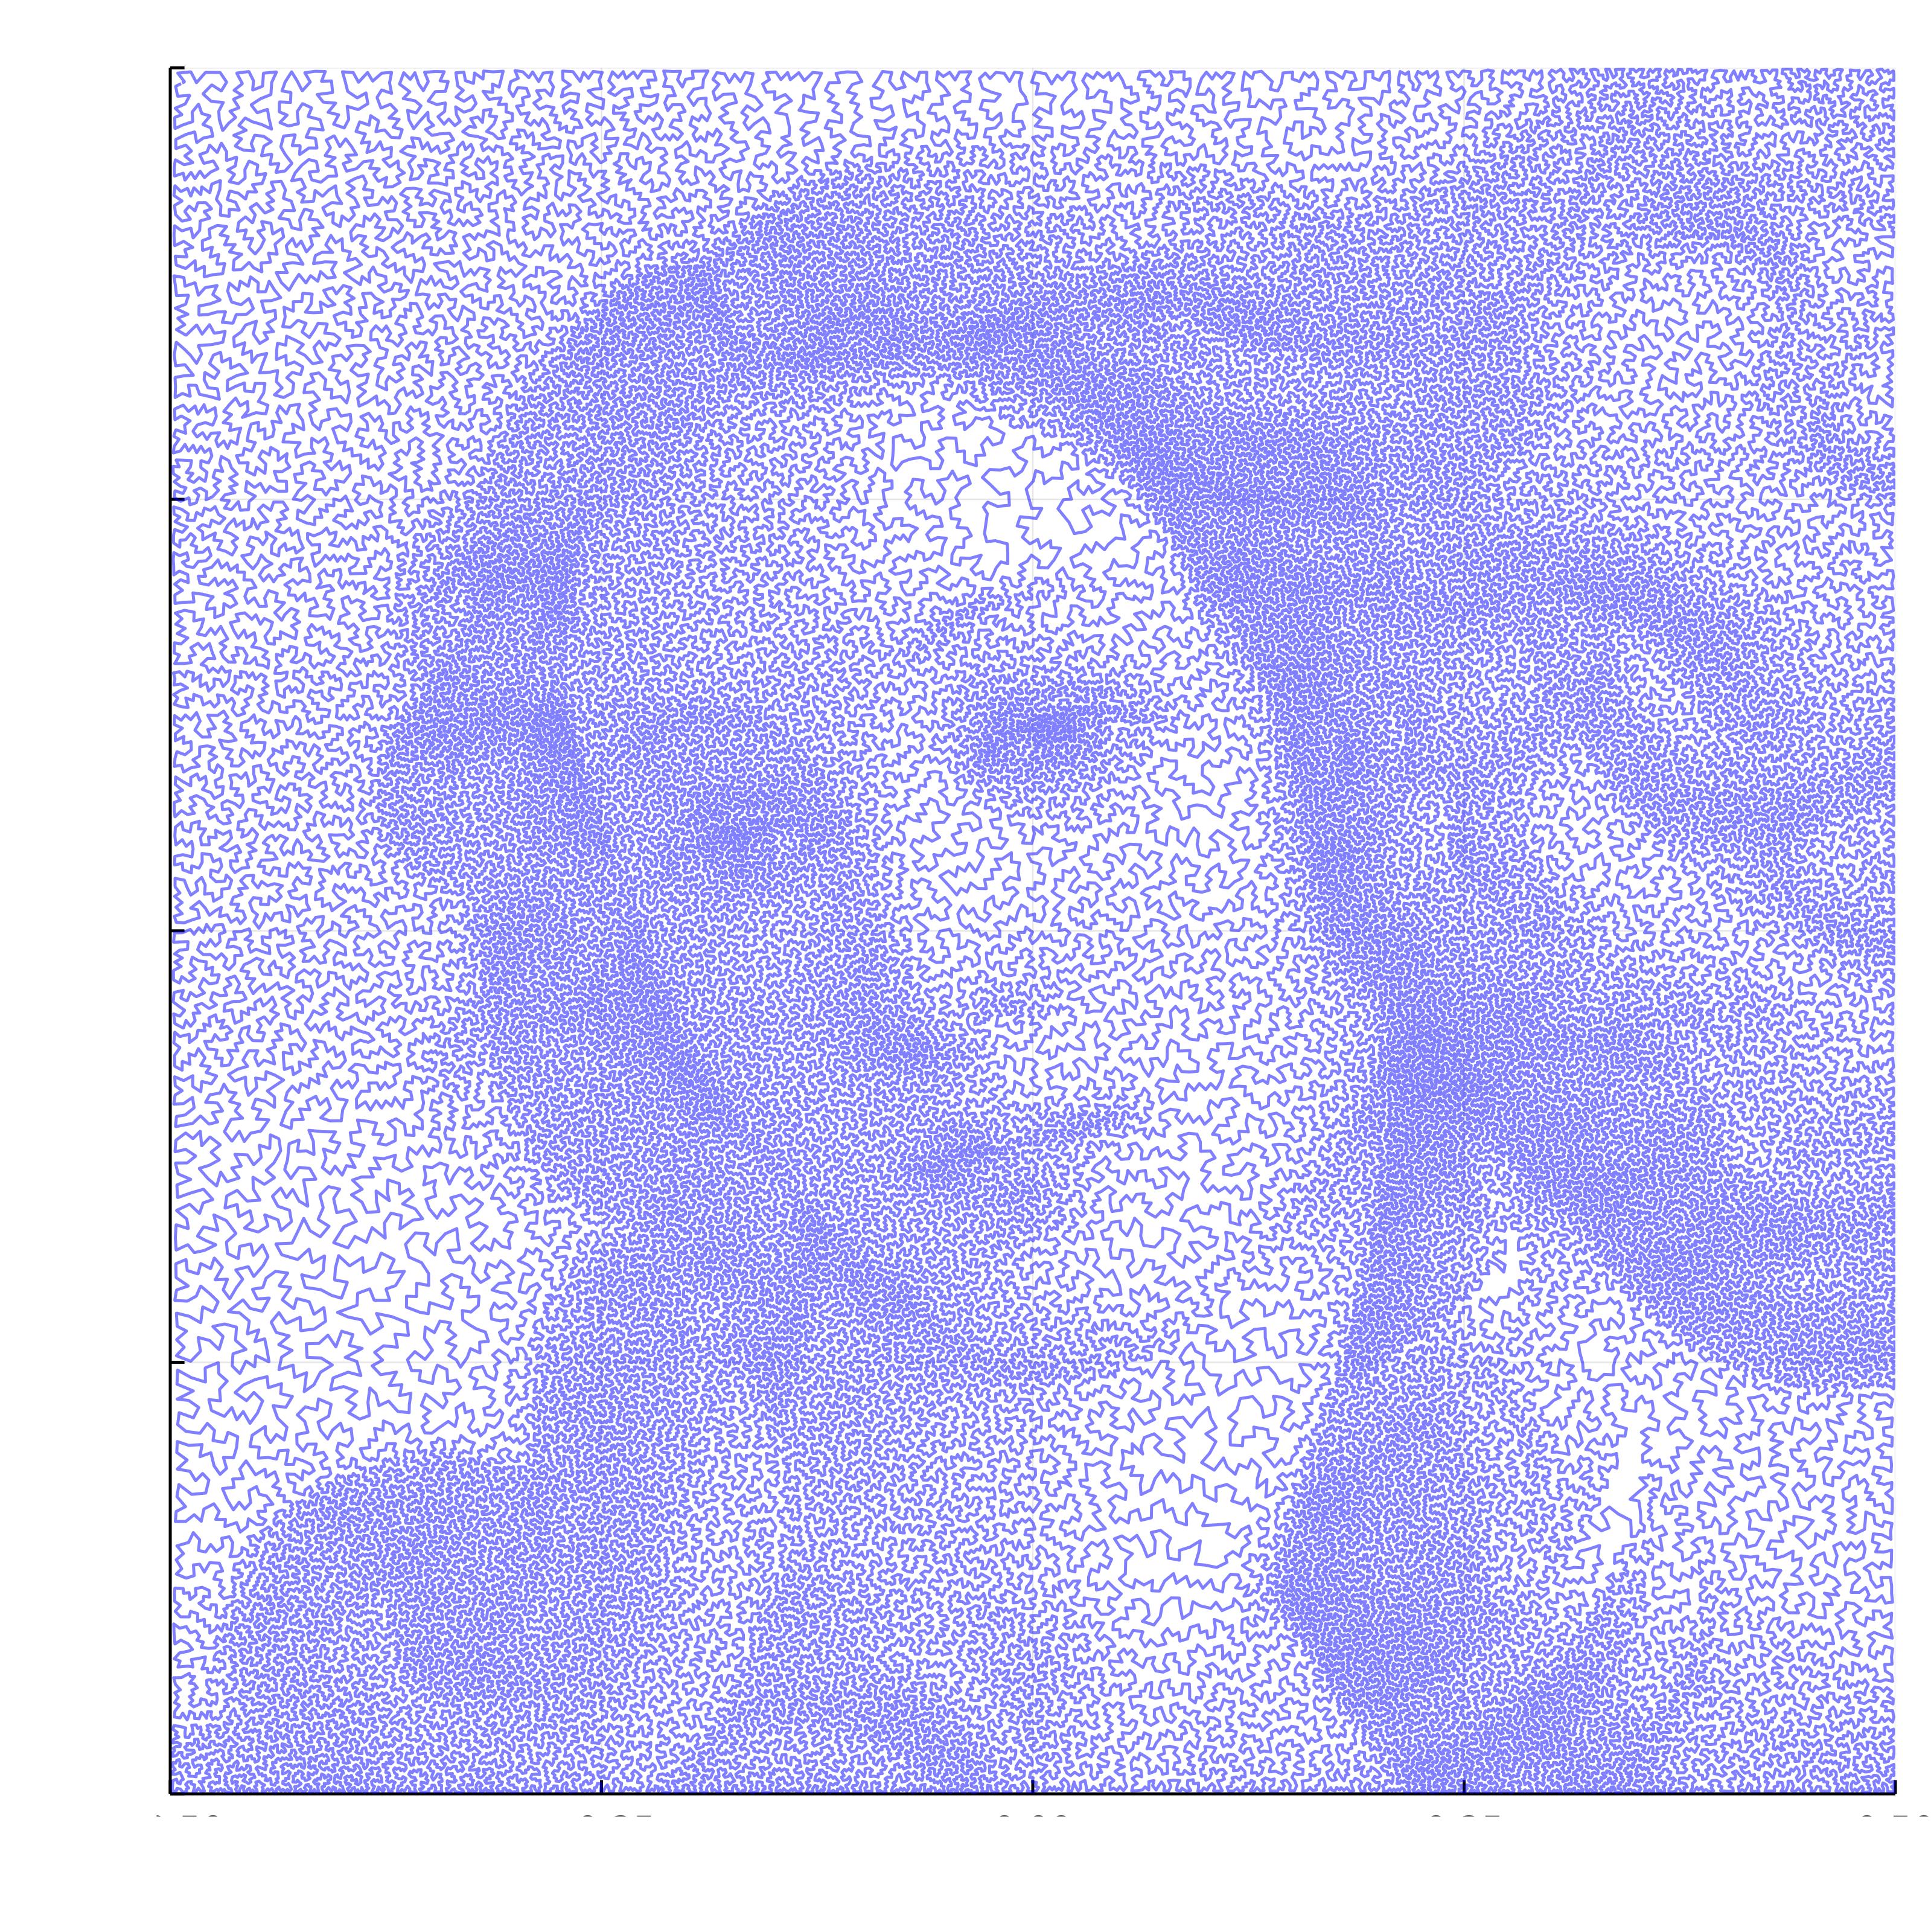
\includegraphics[width=0.9\textwidth]{images/elastic_neighbourhood/fig_3}
\end{figure}
\newpage
\section*{Velazquez's Juan de Pareja}
\begin{figure}[h!]
	\centering
	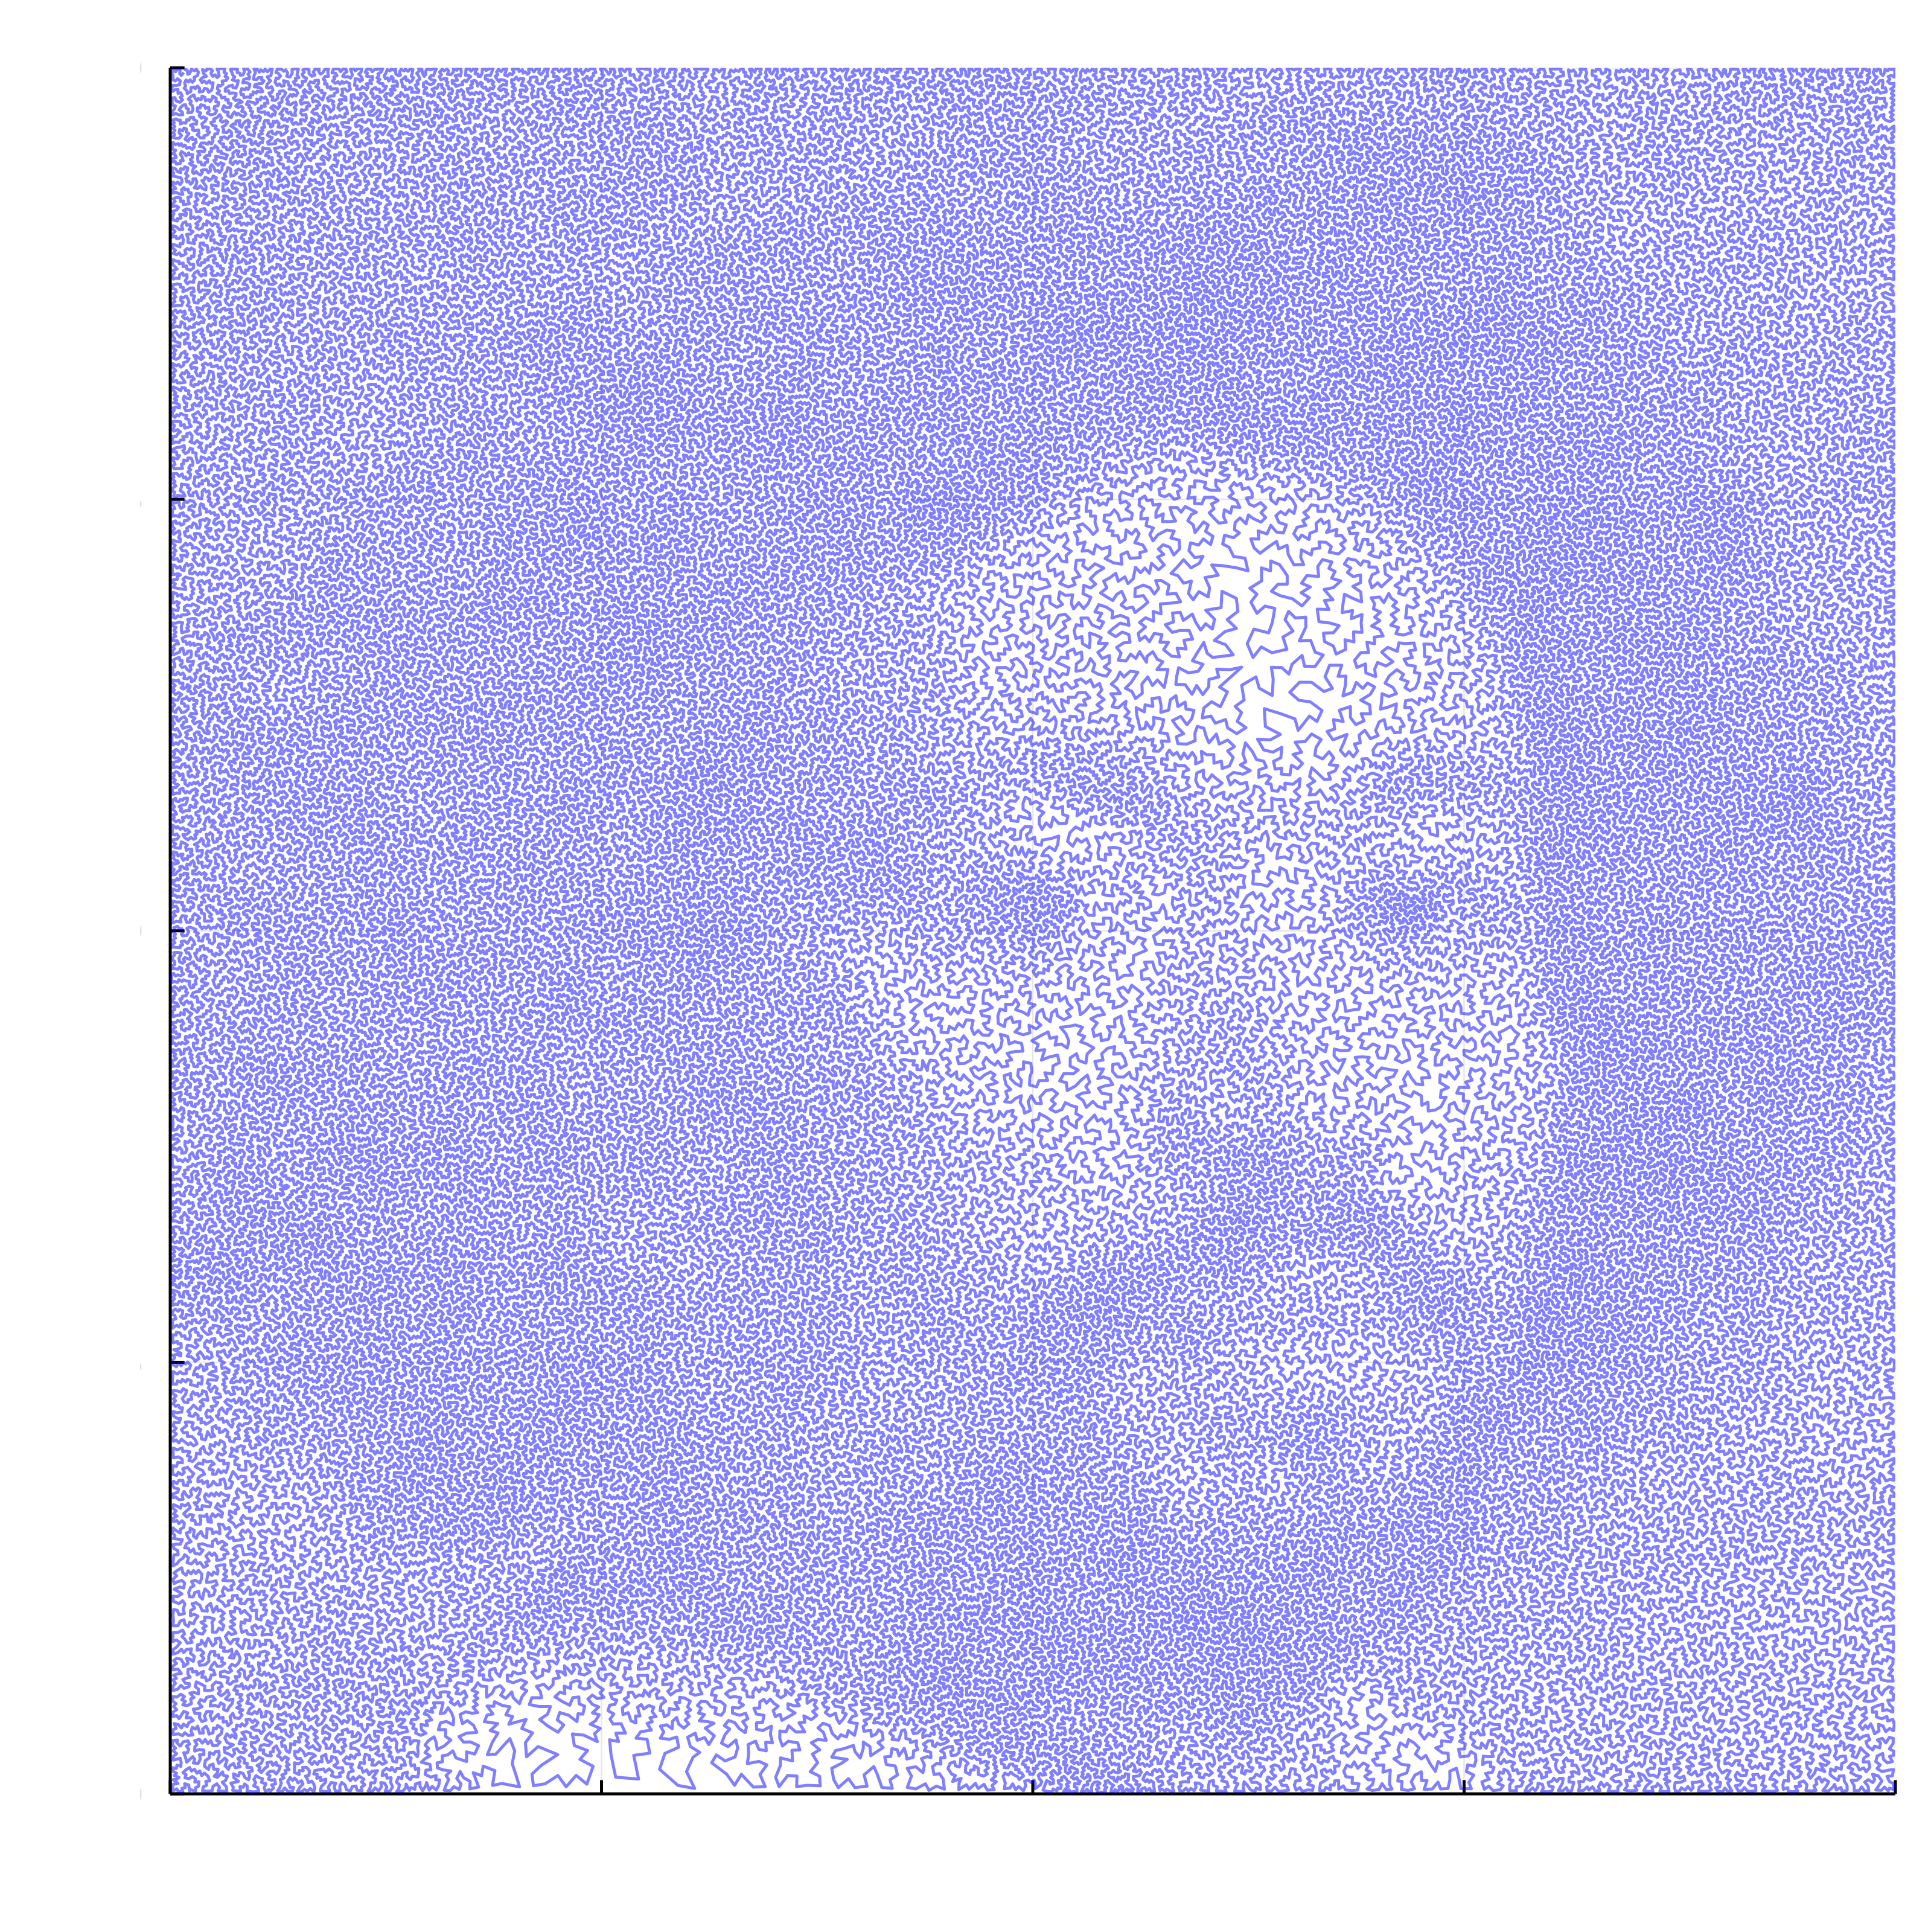
\includegraphics[width=0.9\textwidth]{images/elastic_neighbourhood/fig_4}
\end{figure}
\newpage
\section*{Courbet's The Desperate Man}
\begin{figure}[h!]
	\centering
	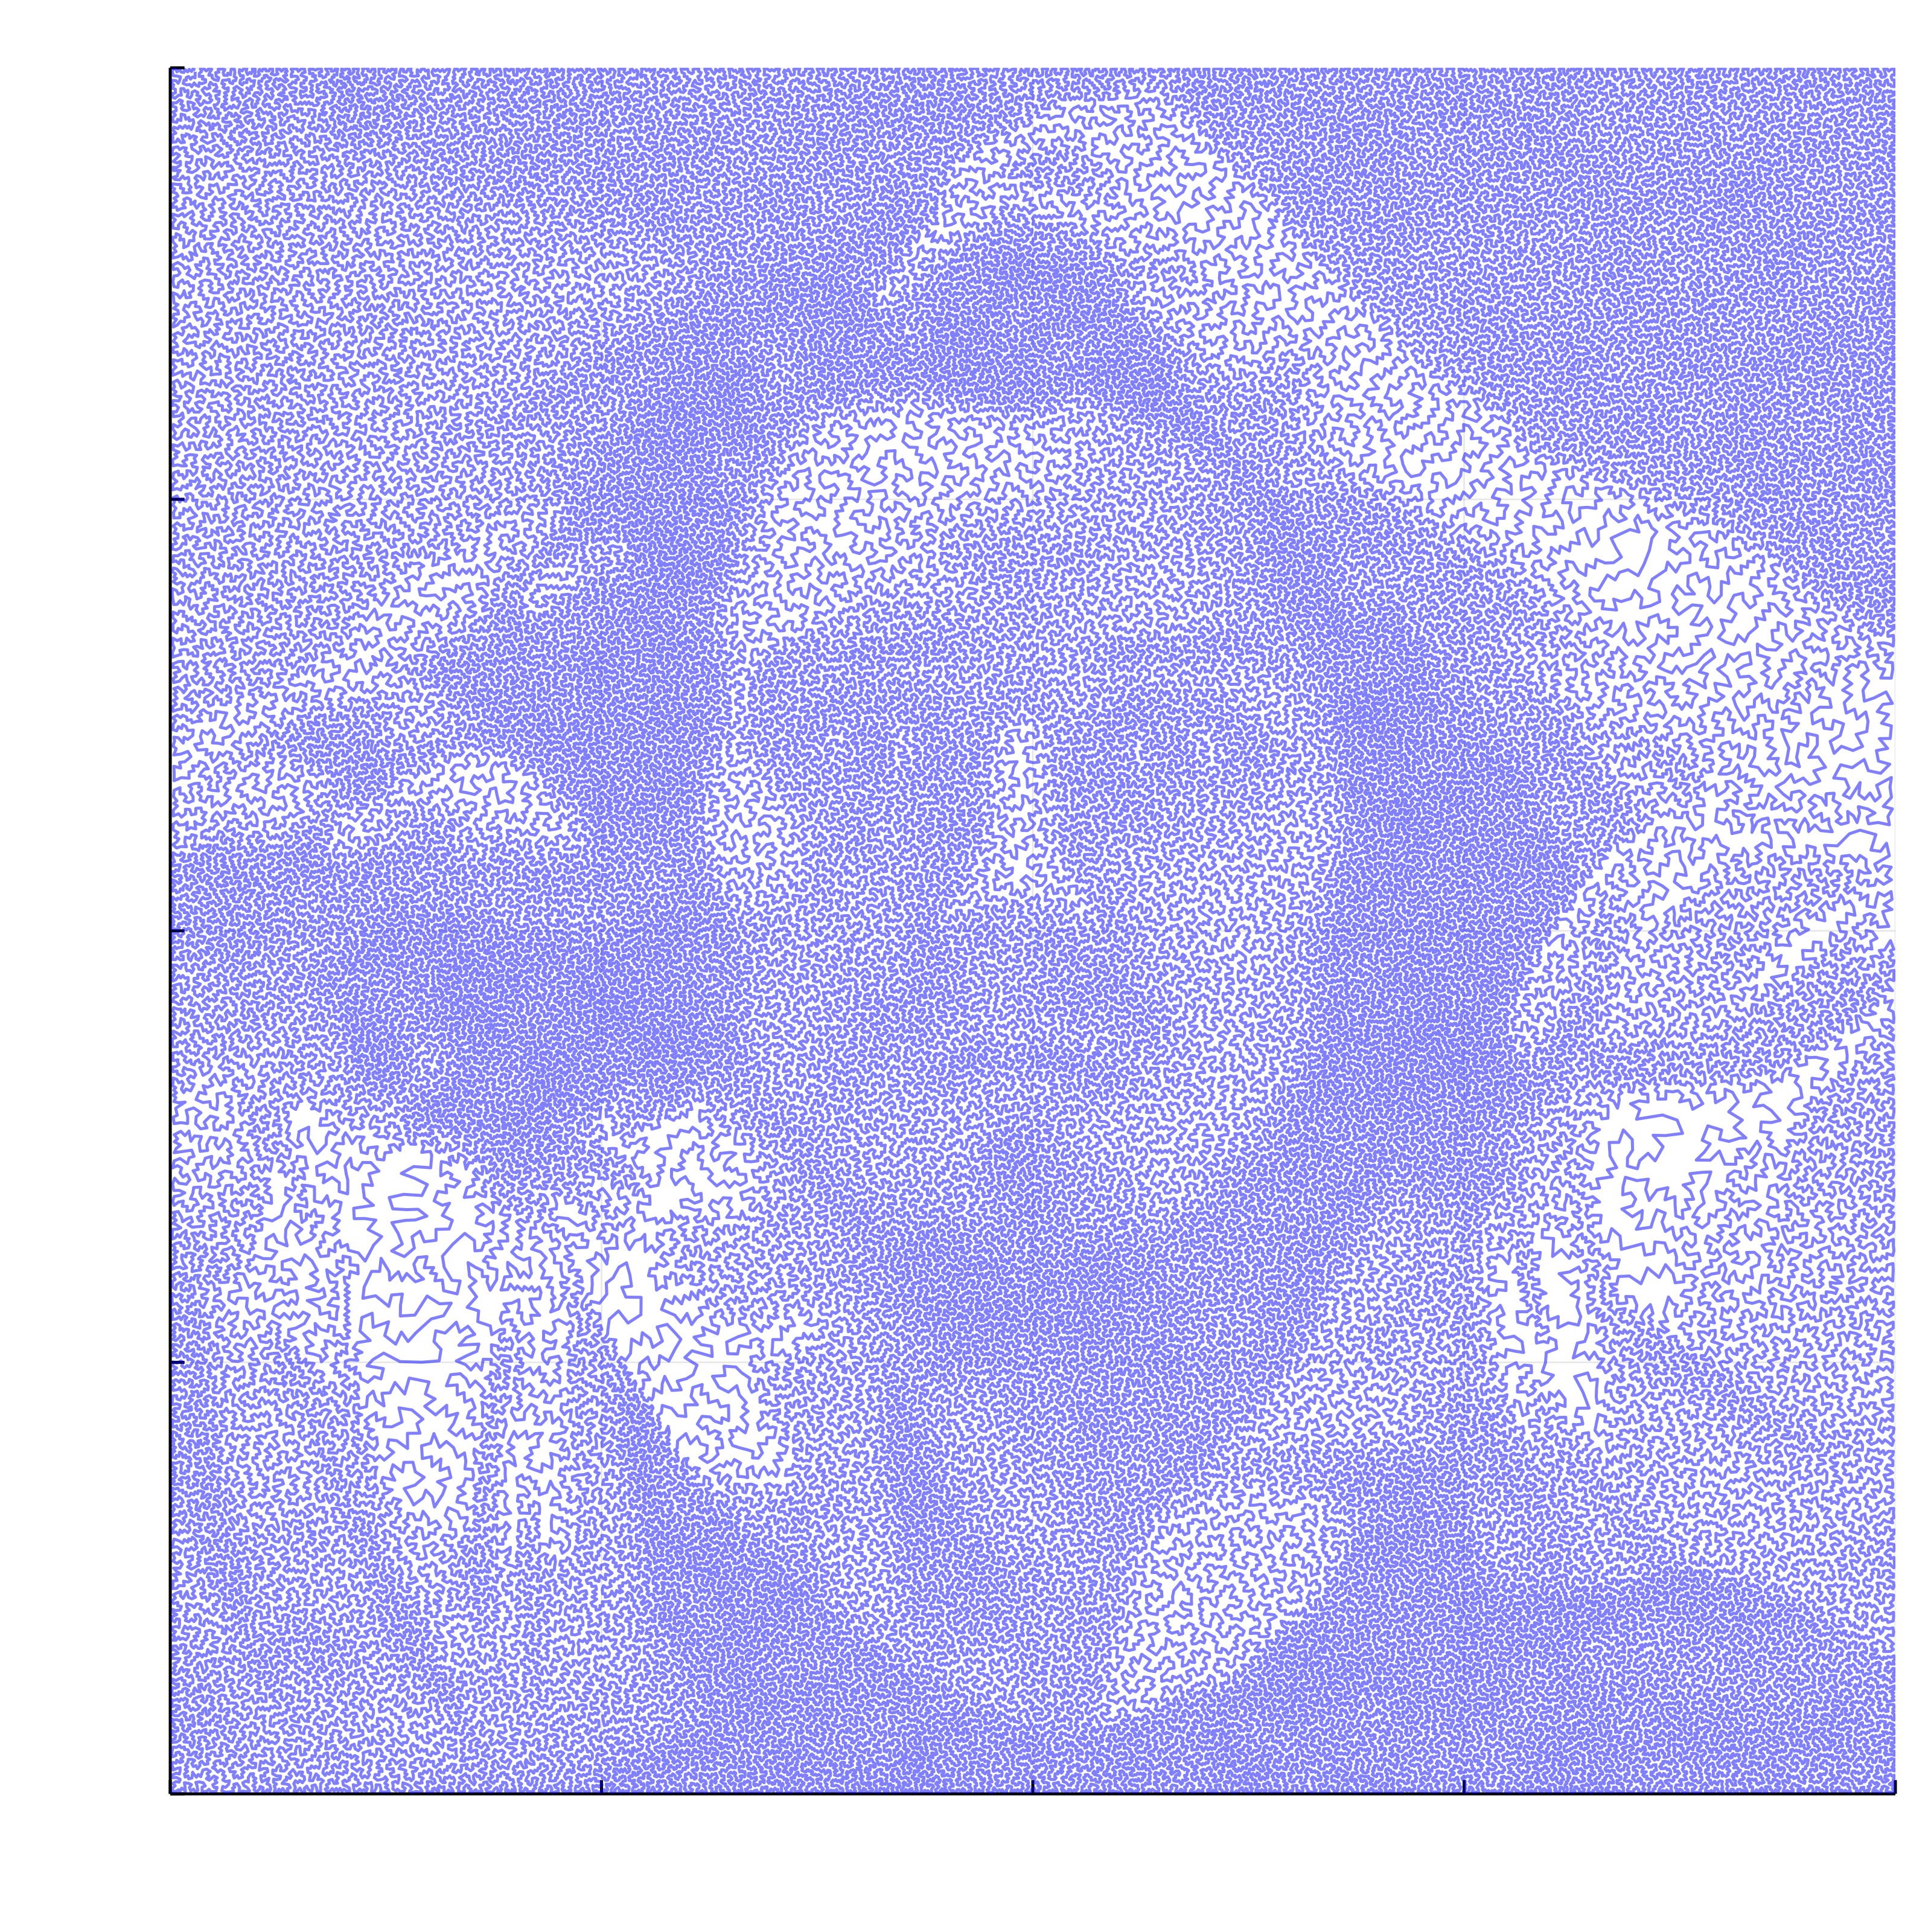
\includegraphics[width=\textwidth]{images/elastic_neighbourhood/fig_5}
\end{figure}
\newpage
\section*{Vermeer's Girl with a Pearl Earring}
\begin{figure}[h!]
	\centering
	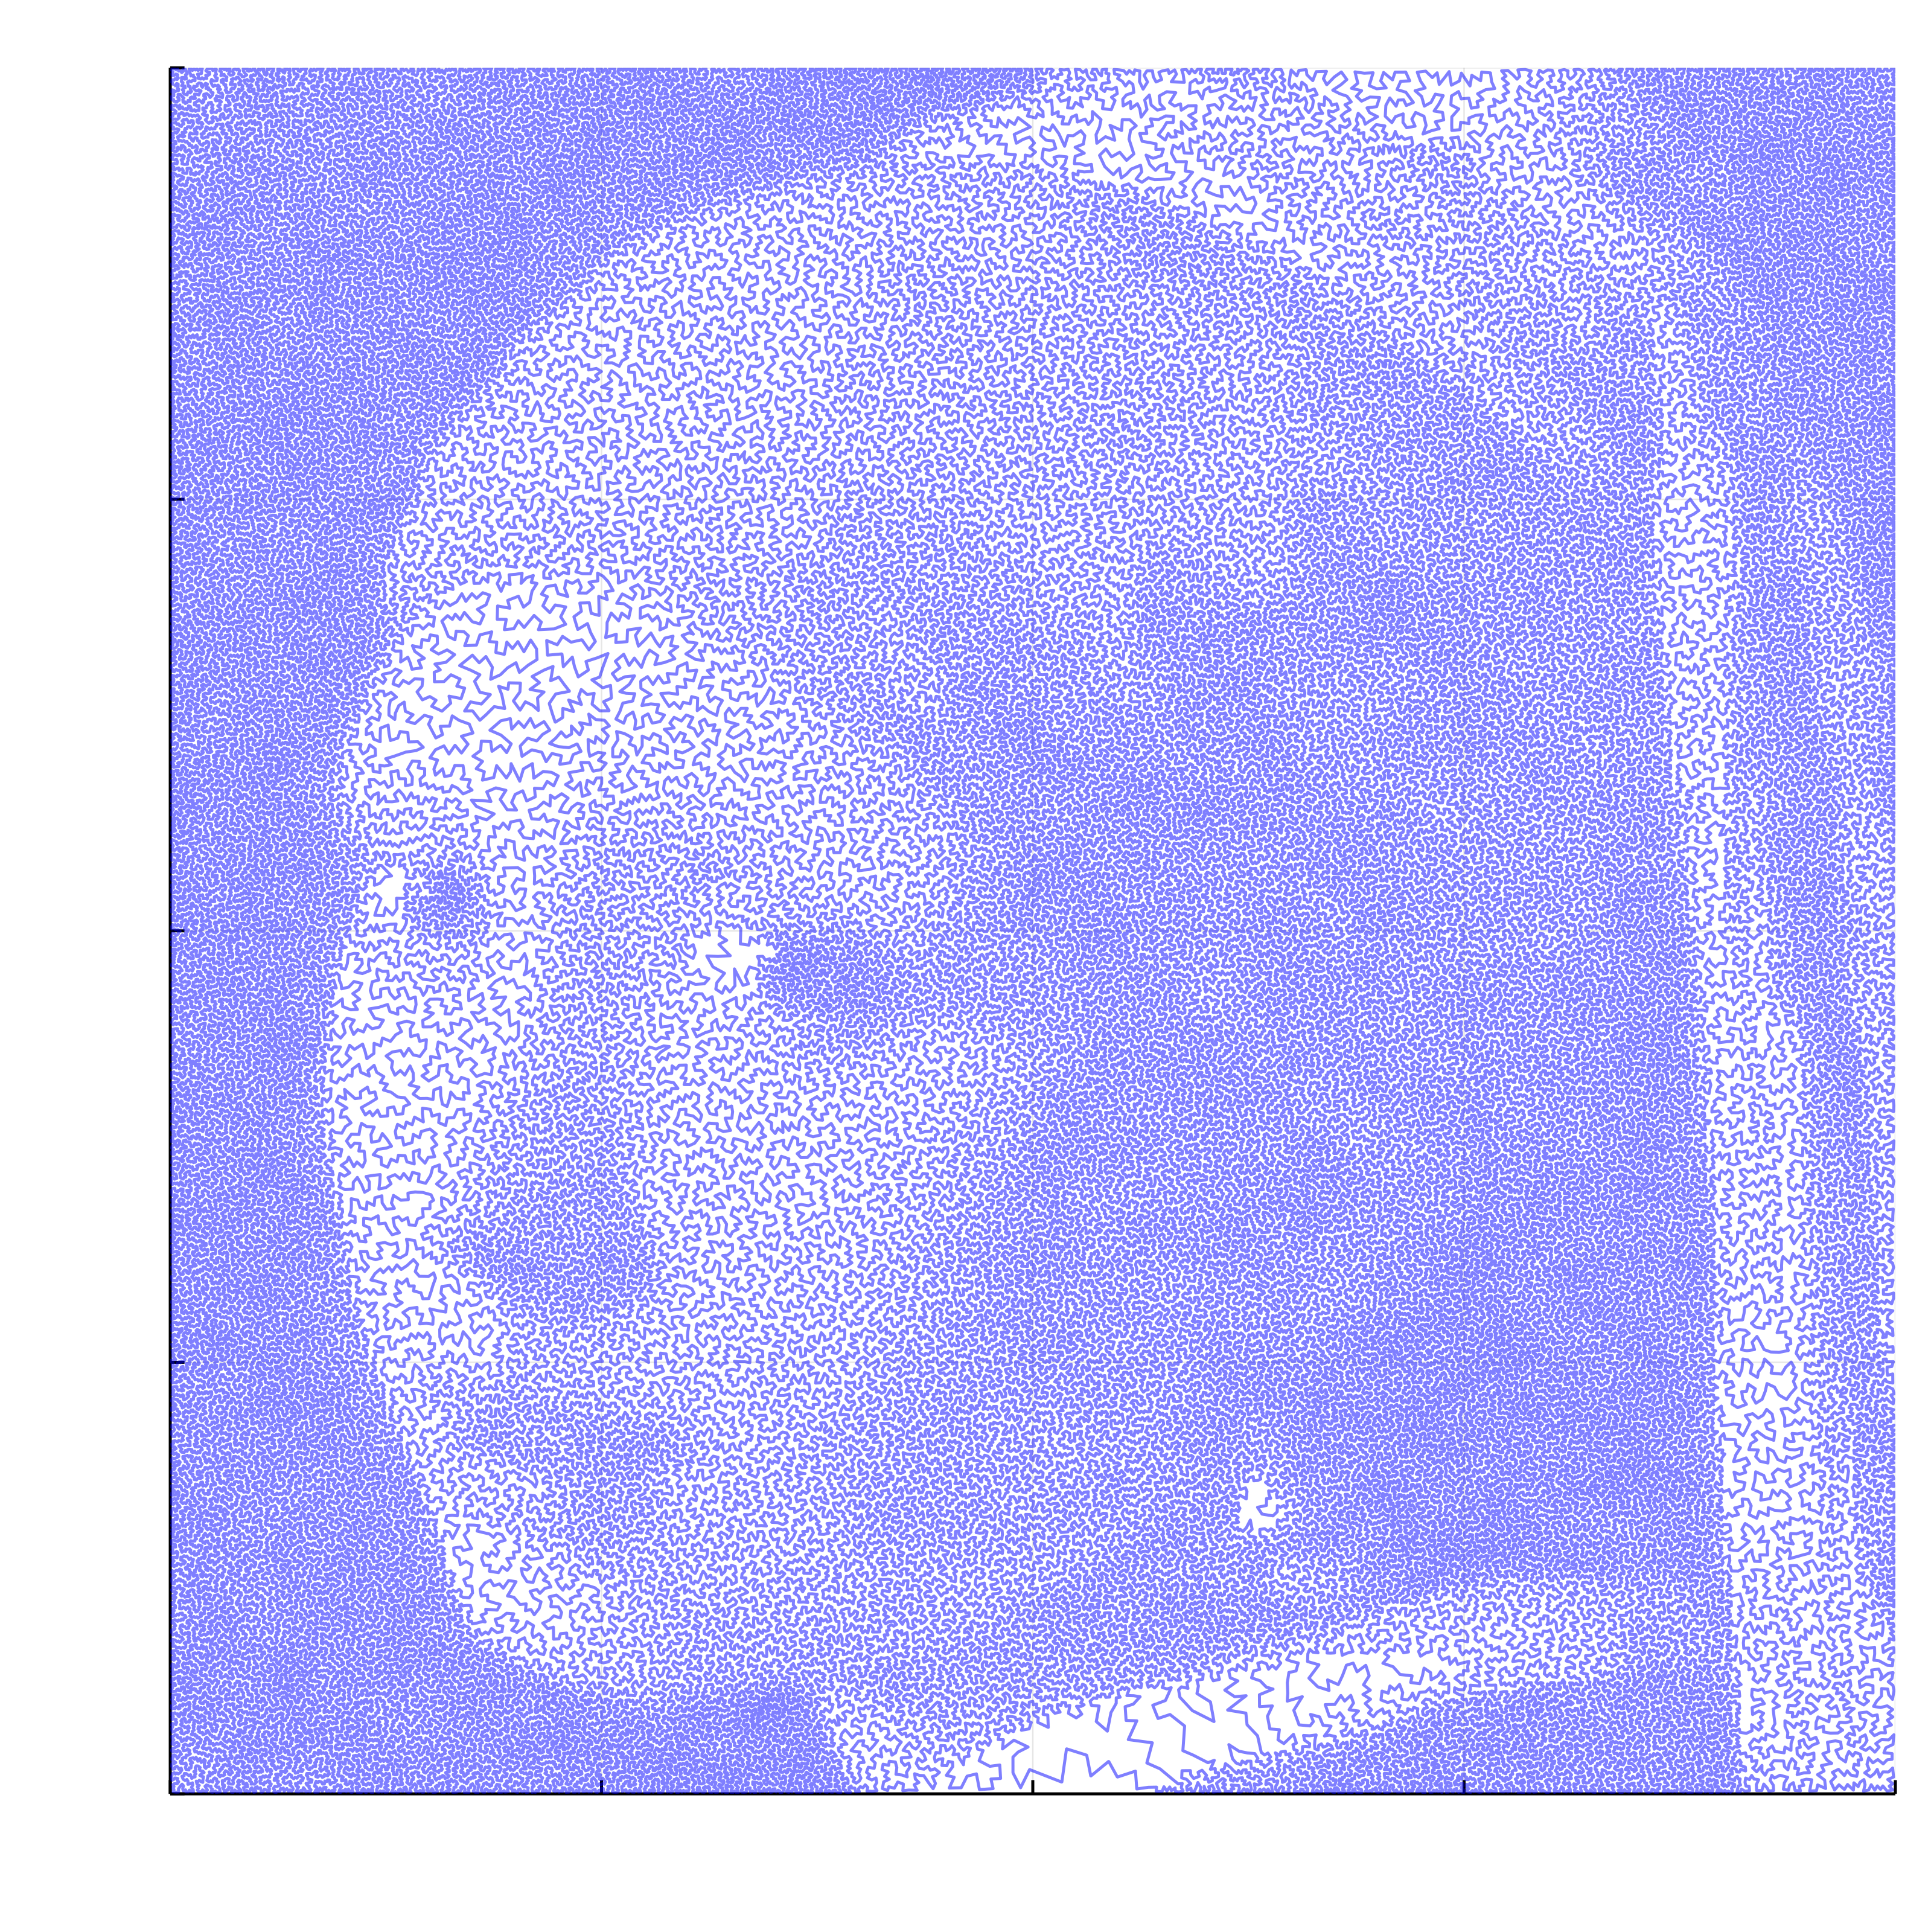
\includegraphics[width=\textwidth]{images/elastic_neighbourhood/fig_6}
\end{figure}